
% PACKAGES INCLUDED HERE 
% DO NOT NEED TO CHANGE
\documentclass[conference]{IEEEtran}
\IEEEoverridecommandlockouts
% The preceding line is only needed to identify funding in the first footnote. If that is unneeded, please comment it out.
\usepackage{cite}
\usepackage{amsmath,amssymb,amsfonts}
\usepackage{algorithmic}
\usepackage{graphicx}
\graphicspath{ {figures/} }
\usepackage{textcomp}
\def\BibTeX{{\rm B\kern-.05em{\sc i\kern-.025em b}\kern-.08em
    T\kern-.1667em\lower.7ex\hbox{E}\kern-.125emX}}
\begin{document}

% AUTHOR NAMES AND TITLE GOES HERE
\title{Towards Rich Word Embedding for Text Generation Using Recurrent Neural Networks}

\author{
\IEEEauthorblockN{Samuel Remedios}
\IEEEauthorblockA{\textit{Department of Computer Science} \\
\textit{Middle Tennessee State University}\\
Murfreesboro, TN, USA \\
swr2u@mtmail.mtsu.edu}

\and

\IEEEauthorblockN{Madison Karrh}
\IEEEauthorblockA{\textit{Department of Computer Science} \\
\textit{Middle Tennessee State University}\\
Murfreesboro, TN, USA \\
mtk2r@mtmail.mtsu.edu}

\and

\IEEEauthorblockN{Michael Schmidt}
\IEEEauthorblockA{\textit{Department of Computer Science} \\
\textit{Middle Tennessee State University}\\
Murfreesboro, TN, USA \\
ms7e@mtmail.mtsu.edu}

\and

\IEEEauthorblockN{Brent Perez}
\IEEEauthorblockA{\textit{Department of Computer Science} \\
\textit{Middle Tennessee State University}\\
Murfreesboro, TN, USA \\
bap4j@mtmail.mtsu.edu}

\and

\IEEEauthorblockN{John Westbrooks}
\IEEEauthorblockA{\textit{Department of Computer Science} \\
\textit{Middle Tennessee State University}\\
Murfreesboro, TN, USA \\
xxxx@mtmail.mtsu.edu}

\and

\IEEEauthorblockN{Joshua Phillips}
\IEEEauthorblockA{\textit{Department of Computer Science} \\
\textit{Middle Tennessee State University}\\
Murfreesboro, TN, USA \\
joshua.phillips@mtsu.edu}
}

\maketitle

% ABSTRACT AND KEYWORDS
\begin{abstract}
Language modeling and text generation have been studied for decades, but more recently deep learning and other machine learning techniques have been applied to these tasks. Although work has been done with Markov modeling and recurrent neural networks (RNNs), not much progress has been made with higher-level linguistic structure such as subject-participle construction or parts of speech.  Our work infuses standard word embedding techniques with the respective part of speech, with the hopes of improving the sensibility of generated text.  We compare structure between this enriched word embedding technique applied to RNNs to word-level Markov chains and non-enriched word embedding-based RNNs.  However, both qualitatively and quantitatively results are disappointing, where none of the proposed methods perform well.  The selected string distance metrics are not sensible as a means of comparing generated text, and more work must be done to improve data preprocessing, metric exploration, model improvements, and feature selection.
\end{abstract}

\begin{IEEEkeywords}
text generation, recurrent neural network, natural language processing, language modeling, computational linguistics, part of speech tagging, word2vec, word embedding
\end{IEEEkeywords}

% SECTIONS
\section{Introduction}
Semantic understanding of natural language has been a difficult problem in computer science for decades. \cite{linell2004written} While many great strides have been made in many subfields such as sentiment analysis \cite{medhat2014sentiment}, word embeddings \cite{DBLP:journals/corr/MikolovSCCD13}, text generation \cite{sutskever2011generating}, classification \cite{dumais2001methods}, and summarization \cite{Goldstein:1999:STD:312624.312665}, there still lacks an effective means of human-level text modeling \cite{WENYIN20104031}\cite{YAN201715}\cite{BICALHO201766}. Recently, more tools have become available to help in this endeavour \cite{DBLP:journals/corr/MikolovSCCD13}\cite{bird2004nltk}\cite{honnibal2015improved}, and the aggregation of techniques is now possible. One such example is the generation of a caption given an image \cite{johnson2016densecap}, which uses a convolutional neural network in tandem with an RNN and is trained on parsed and tokenized natural language data.  This method utilizes dependency trees as a way of building vectors which embeds the word with its respective part of speech context at once, as well as incorporating neighboring words and their contexts.

Currently, the more popular generative methods aim to model languages from the character-level upwards rather than from the word-level. Even those that operate on a word-by-word basis such as Markov chain modeling \cite{conroy2001text} and n-gram modeling \cite{masataki1996variable} may not incorporate parts of speech nor long-term memory. Traditionally, these word-level models are stochastic; that is, they construct internal representations of language by building a probabilistic mapping between previous words in the sequence to the current word. However, natural language is a complex system\cite{beckner2009language} and thus has more depth than the surface-level words present, such as semantics, grammar, parts of speech, etc, and it would be advantageous to encode this information alongside the words themselves.

For this paper, we evaluate the efficacy of tokenizing words alongside their parts of speech with unique identifiers for use in a recurrent neural network (RNN). Specifically, we aim to generate text using the long short-term memory (LSTM) variant of the RNN using training data comprised of a subset of a scripts from the contemporary popular American cartoon television show, Rick and Morty. This method of encoding natural language has an advantage over the previously mentioned dependency trees by being fully transparent and customizable for the user; it is for example possible to manually change the embedding of the parts of speech, the words themselves, or to add more language features as needed in order to achieve the desired goal.

\section{Methods}

\subsection{Data}

The data used in this study was a short subset of a transcript found online\cite{rickandmorty} from the American television series Rick and Morty. We arbitrarily gathered $50$ sequential sentences from the first episode of Rick and Morty. The number of total words, unique words, and outlier words in our dataset are outlined in Table \ref{tab:data}, where an outlier word is defined as any word with a frequence of less than $5$ occurrences.

\begin{table}[!htbp]
\caption{Dataset statistics. $50$ total sentences were used. An uncommon word is defined as a word which occurs less than $5$ times.}
\label{tab:data}
\begin{center}
\begin{tabular}{lccc}

Series & Total Words & Unique Words & Uncommon Words\\
\hline{}\\
Rick and Morty & $649$ & $220$ & $21$\\

\end{tabular}
\end{center}
\vspace{-1em}
\end{table}

\subsection{Preprocessing}

As the data was found via an online source, there was much heterogeneity in the scripts.  We therefore had several cleaning steps to ensure the data could be handled by our model properly.  First we programmatically split sentences by the presence of end-of-sentence delimiters such as ".", "!", and "?", but without taking into account non-terminal punctuation such as the periods in "Dr.", "Mrs.", and "Mr.".  Next, we removed extraneous white space, then set the case of all character to be lower.  The starts of all sentences were then verified to start with words rather than symbols such as "-" or spaces, and finally we appended special "ST" and "EN" tokens to the beginnings and ends of each sentence, to allow the model to easily learn when sentences should begin and end.

We encoded each unique word into a one-hot vector such that each word was represented by a single $244$-dimensional sparse vector in which only a single element is set to $1$ and $0$ for the rest.  We then used NLTK \cite{bird2004nltk} to generate the appropriate part of speech tag for every word in our corpus, converted this tag into a one-hot vector of length $47$ and subsequently mapped each word into its respective one-hot space.  To finalize preprocessing, we concatenated the one-hot vector representing the word with the one-hot vector representing the part of speech, resulting in a $291$-element vector.

\subsection{Recurrent Neural Network Architecture}

The model selected for this problem was an RNN model comprised of a fully-connected layer leading into two LSTM layers and finally into one fully-connected layer of size $244$, corresponding to the length of the one-hot word vector, which was subsequently activated with the softmax function.  As this is a classification problem, we used categorical crossentropy as our loss.  To aid with learning, we utilized a LeakyReLU activation before the LSTM layers, allowing gradient values below $0$ to flow through to the prior layer.  The model is depicted in Figure \ref{fig:model}.

\begin{figure}[!htbp]
\caption{RNN architecture.  The word and part of speech vectors are concatenated prior to being fed into the network. Noise is supplied to the network in parallel, then is added element-wise to the data vector. The signal subsequently flows through a fully-connected (dense) layer, LeakyReLU activation, two LSTMs, and two final fully-connected layers where the final activation is softmax.}
\label{fig:model}
\centering
\vspace{2mm}
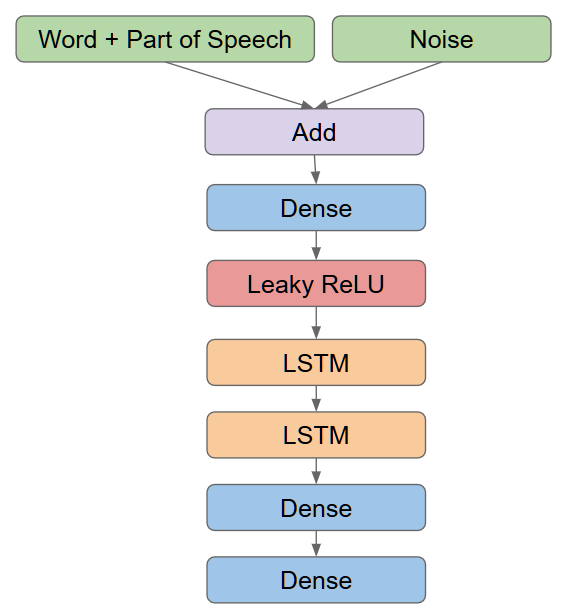
\includegraphics[scale=0.5]{rnn}
\end{figure}
Since neural networks are deterministic models, text generation is prone to falling into a so-called loop, where the model may map $A$ to $B$, $B$ to $C$, and $C$ to $A$.  To avoid this, we supplied the network with an auxiliary input vector of equal length to the word and part of speech vector.  This auxiliary input has random entries pulled from the Gaussian standard normal distribution, linearly scaled down by a factor of $10$ such that entries were $\in[-0.1, 0.1]$.  To allow for this auxiliary input, our model takes an independent input, then performs an element-wise sum with the word and part of speech vector before feeding the tensor into the first fully-connected layer.

\subsection{Training and Text Generation}

For training, we supplied the network with $10$ sequential words and provided as ground truth each of those words' subsequent words.  We trained for an arbitrary $10 000$ epochs with a batch size of $50$; in other words, we used our entire training set as our batch size.

To generate text, we defined a sentence to be the existence of the `EN` tag.  We first supplied the network with the one-hot encoding for the start token `ST` alongside the random auxiliary vector, and used the above-described method to feed the model's predictions back as inputs.  By this approach we generated words until the `EN` tag appeared $50$ times, thus matching the number of "sentences" as in our dataset.


\subsection{Postprocessing}

The output of the RNN is a $244$-element vector corresponding to the previously-mentioned one-hot encoding.  To map this output back into word space, we calculated the vector distances between our output and each word vector in our dataset to find the closest match.  We then wrote the corresponding word to a file, and used the exact one-hot encoding for the closest word as input for the RNN to generate its next output.  We also find the part of speech of the closest word, and concatenate it to the one-hot encoding as done during preprocessing. In this manner, the RNN always takes the two concatenated one-hot encodings in as its input, despite it generating dense vectors as output.

\section{Results}
To validate our model, we compared it to two other methods: a word-level Markov chain and the same word-level RNN without part of speech embeddings.  Qualitative results are shown in \ref{fig:qual_results}, where the two most realistic sentences from each model were chosen.

\begin{figure}[ht]
\caption{Two example sentences as qualitative results from each of the Markov Chain, word-RNN (w-RNN), and enriched word-RNN (e-RNN) models. These are the subjectively best sentences picked by human raters.}
\label{fig:qual_results}
\centering
\vspace{2mm}
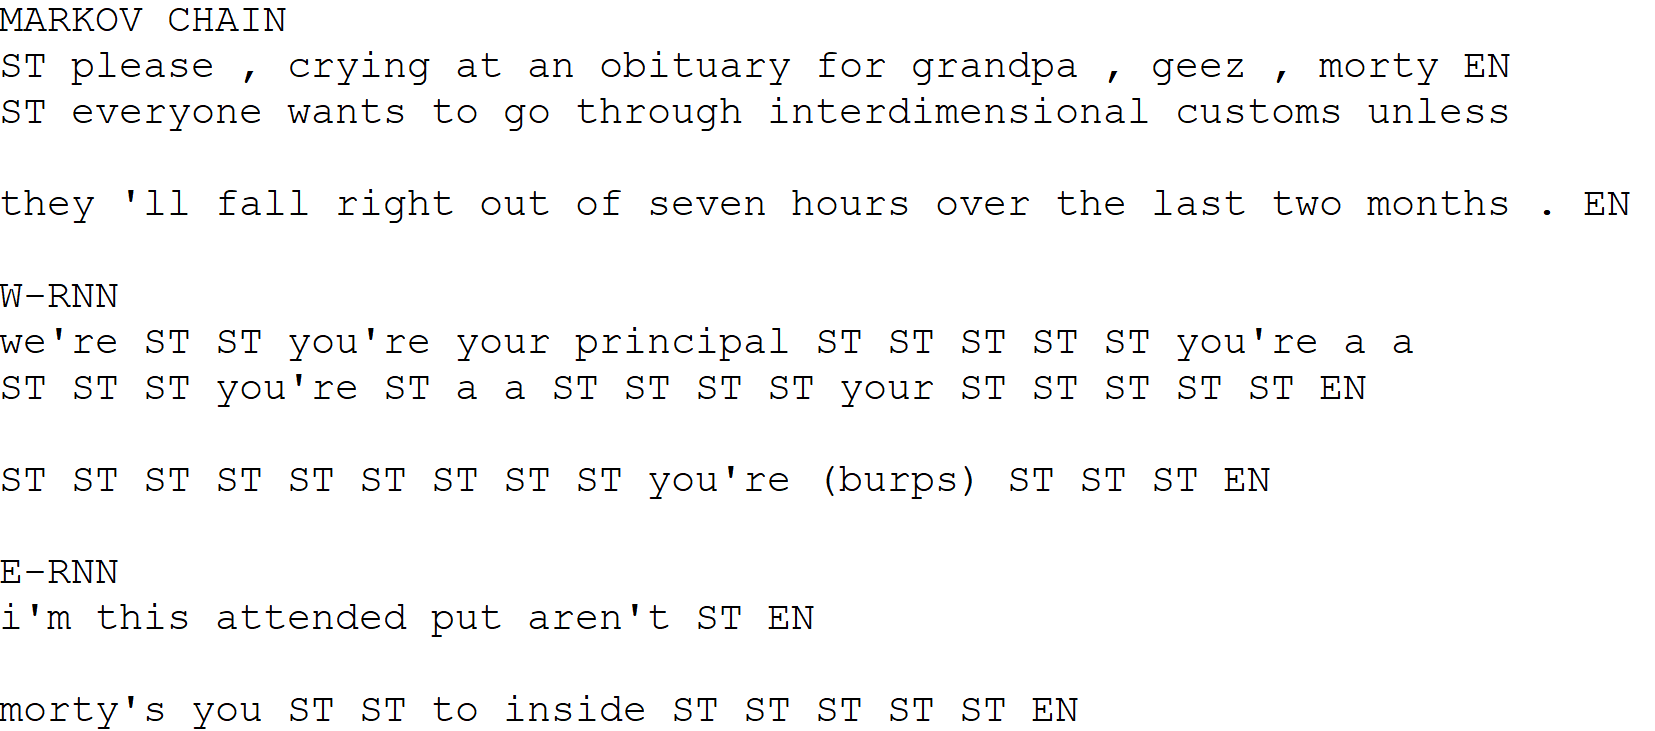
\includegraphics[scale=0.2]{qualitative_examples}
\end{figure}

For quantitative comparison, we used $4$ different known string comparison metrics\cite{cohen2003comparison} over the resulting parts of speech of each of the $3$ method's output.  Specifically, for each sentence in the outputs of each of the Markov chain (MC), the word-RNN (w-RNN) and the enriched word-RNN (e-RNN) were part of speech tagged, and these tags were compared to the original dataset's part of speech tags using Hamming distance\cite{norouzi2012hamming}, cosine similarity\cite{cohen2003comparison}, Gotoh's algorithm\cite{gotoh1982improved}, and Levenshtein distance\cite{yujian2007normalized}.  These $50$ measured distances were then averaged to produce the results seen in Table \ref{tab:results_table}

The Hamming distance measures the number of differences between a pair of strings.  In this circumstance, this is the number of mismatches between the parts of speech in the original data and each of the generated samples. With regards to tokenized natural language, cosine similarity measures distances as vectors according to the formula:
$$similarity = \frac{\sum_{i=1}^{n}A_iB_i}{\sqrt{\sum_{i=1}^{n}A_i^2}\sqrt{\sum_{i=1}^{n}B_i^2}} $$ Gotoh's algorithm originally was proposed as a more efficient means of comparing biological sequences, but can also be applied to natural language.  Finally, similar to Hamming distance, Levenshtein distance measures mismatches of arbitrary length.

\begin{figure}[ht]
\caption{Training curve for data without parts of speech appended. Accuracy is $\in[0,1]$ and represents the accuracy with which the model correctly selects the next words in the sequence.}
\label{fig:curve_without_pos}
\centering
\vspace{2mm}
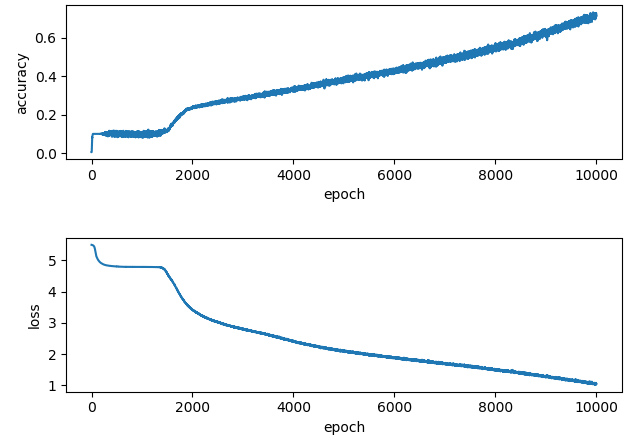
\includegraphics[scale=0.5]{training_curve_without_pos}
\end{figure}

\begin{figure}[ht]
\caption{Training curve for data with parts of speech appended. Accuracy is $\in[0,1]$ and represents the accuracy with which the model correctly selects the next words in the sequence.}
\label{fig:curve_with_pos}
\centering
\vspace{2mm}
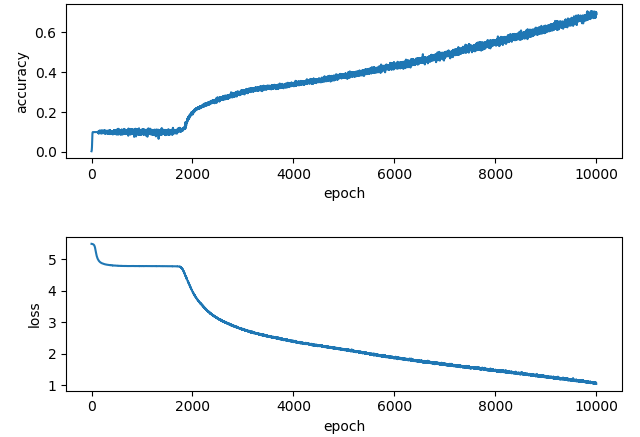
\includegraphics[scale=0.5]{training_curve_with_pos}
\end{figure}




\begin{table}[!htbp]
\caption{Distance metrics between generated corpus and the original corpus.  For comparison, the distance of the ground truth compared against itself is shown.  Best results are highlighted in bold, excluding the ground truth.}
\label{tab:results_table}
\begin{center}
\begin{tabular}{lcccc}

Metric & Ground Truth & MC & w-RNN & e-RNN\\
\hline{}\\
Hamming & $0$ & $3.901$ & $4.439$ & $\textbf{3.427}$\\
Cosine & $0.05$ & $0.035$ & $0.030$ & $\textbf{0.0296}$\\
Gotoh & $3.732$ & $\textbf{1.225}$ & $0.347$ & $0.119$\\
Levenshtein & $0$ & $\textbf{2.532}$ & $3.301$ & $2.684$\\

\end{tabular}
\end{center}
\vspace{-1em}
\end{table}


\section{Discussion}

Although we did see an improvement both qualitatively and quantitatively with the inclusion of parts of speech in RNNs, overall results are disappointing.  Subjectively inspecting the output data as a human rater, the sentences generated by both variants of the RNN failed.  Additionally, while the quantitative results from distances between parts of speech look promising, the apparent dichotomy between the chosen string comparison metrics and the actual generated text demonstrates that metrics alone are not sufficient to capture the complexities of natural language.  Even the training curves with and without the part of speech features are very similar, where the loss dips a couple hundred epochs earlier without the parts of speech.  This is sensible though, as with fewer elements in the input vector the model can converge quicker.

Future work in the application of deep learning to natural language generation includes exploring better quantitative metrics, more attention towards RNN architecture design and hyperparameter choice, more directed efforts with respect to data preprocessing, and investigation of choices of alternative text encodings such as using word2vec or other grammatical or semantic features as auxiliary inputs.

\section*{Acknowledgment}

We'd like to thank the Department of Computer Science at Middle Tennessee State University and Joshua Phillips for giving us the opportunity to perform this research during the CSCI 4850-5850 course.


\bibliographystyle{IEEEtran}
\bibliography{References}

\end{document}